\section{Self-attention layer}\label{sec:self-attnt-backprop_appendix}





\begin{figure}
    \centering
    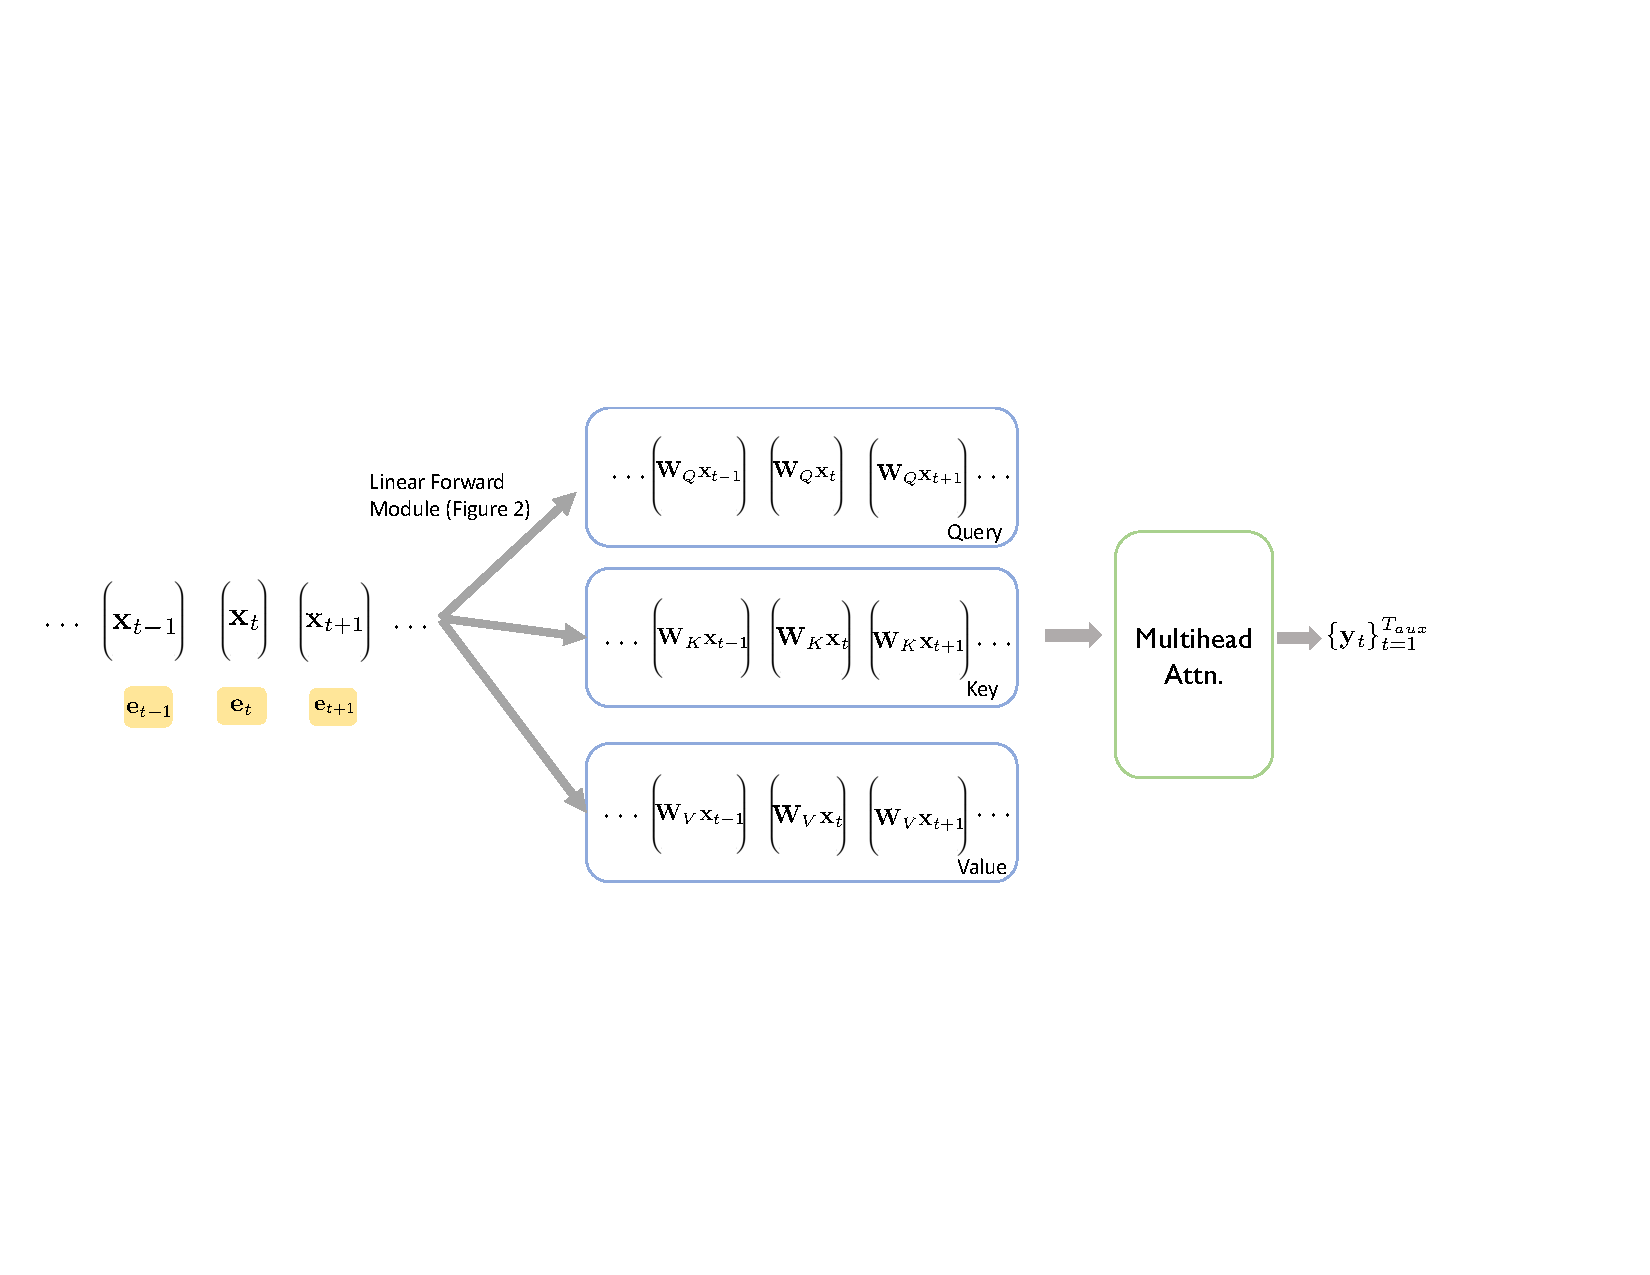
\includegraphics[width=\textwidth]{figures/Attn_forward.pdf}
    \caption{\simulator{} simulates the forward pass of a self-attention layer of the auxiliary model with a Linear Forward module (\cref{fig:linear_forward}) and a \simulator{} softmax attention layer (\cref{def:self-attn_construct}). The Linear Forward module computes the query, key, and value vectors using a Linear Forward module on the current embeddings, changing the prefix embeddings to correspond to $\mW_Q$, $\mW_K$, and $\mW_K$ respectively.}
    \label{fig:attn_forward}
\end{figure}

\begin{figure}
    \centering
    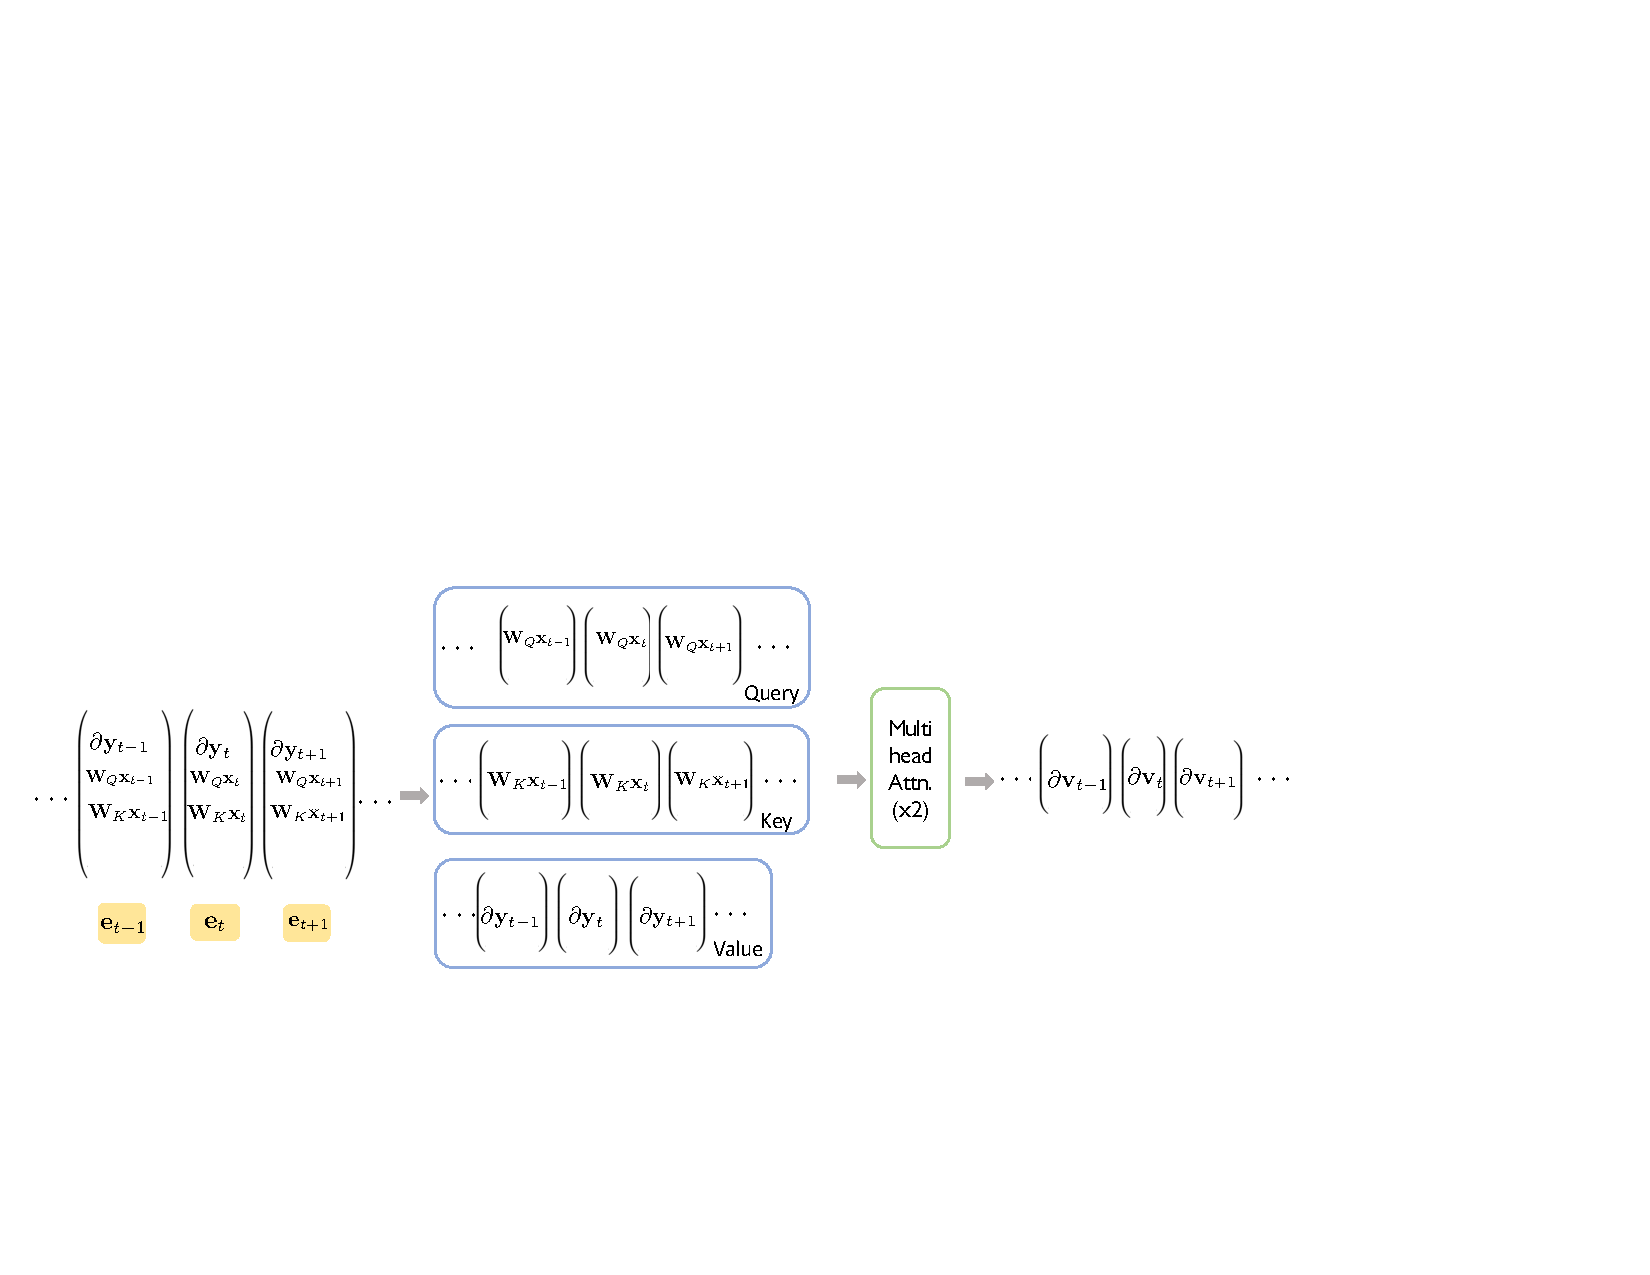
\includegraphics[width=\textwidth]{figures/Attn_valuegradient.pdf}
\caption{The gradient w.r.t. the value vectors $\{\losspartial{\vv_t}\}$  (\cref{def:self-attn-backprop}) forms the integral component for both \simulator{} self-attention backward and descent update modules. \simulator{} computes $\{\losspartial{\vv_t}\}$ using a softmax attention and a linear attention layer. We first use residual connections to copy the query and key vectors to the current embeddings from the \simulator{} Self-attention Forward module (\cref{fig:attn_forward}). The  softmax attention layer re-computes the attention scores $\{a^h_{t, j}\}$ between all token pairs $\{(t, j)\}$ and stores them in the token embeddings. The linear attention layer uses the one-hot position embeddings of the input tokens as the query to use the transposed attention scores $\{a^h_{j, t}\}$ for all token pairs $\{(t, j)\}$ and use the gradients  $\{\losspartial{\vy_t}\}$ as the value vectors to compute $\{\losspartial{\vv_t}\}$.}
    \label{fig:value_gradient}
\end{figure}




We first introduce multi-head attention,  generalizing  single-head attention (\cref{def:self-attn_auxiliary_single}). 
\begin{definition}[Auxiliary self-attention with $\aux{H}$ heads]\label{def:self-attn}
    For query, key, and value weights $\mW_Q, \mW_K, \mW_V \in\RR^{\aux{D}\times \aux{D}}$ and bias $\vb_{Q}, \vb_{K}, \vb_{V} \in\RR^{\aux{D}}$, a self-attention layer with $\aux{H}$ attention heads and a function $\attnfn: \RR^{\aux{T}} \to \RR^{\aux{T}}$ takes a sequence $\{\vx_t\in\RR^{\aux{D}}\}_{t \le \aux{T}}$ as input and outputs $\{ \vy_t \}_{t \le \aux{T}}$, with 
    \begin{align}
        \vy_t = \attmerge ( \{ \sum_{j \le \aux{T}} a^h_{t, j}  \vv^{h}_j  \}_{h \le \aux{H}} ).  \label{eq:attnt_forward}
    \end{align}
    $a^{h}_{t, j}$ is defined as the attention score of head $h$ between tokens at positions $t$ and $j$, and is given by
    \begin{align} \label{eq:attn}
        a^h_{t, j} =  \mathrm{softmax} ( \mK^{h} \vq^{h}_t )_j.
    \end{align}
     Here, $\vq_t$, $\vk_t$, $\vv_t$ denote the query, key, and value vectors at each position $t$, computed as $\mW_Q \vx_t + \vb_Q$, $\mW_K \vx_t + \vb_K$, and $\mW_V \vx_t + \vb_V$ respectively. In addition, $\vq^{h}_t, \vk^{h}_t, \vv^{h}_t$ denote $\attsplit_{\aux{H}} (\vq_t)_h$, $\attsplit_{\aux{H}} (\vk_t)_h$, and $\attsplit_{\aux{H}} (\vv_t)_h$ respectively for all $t \le \aux{T}$, and $h \le \aux{H}$. 
     $\mK^h \in \RR^{\aux{T} \times \aux{D} }$ is defined with its rows as $\{\vk^h_t\}_{t \le \aux{T}}$ for all $h \le \aux{H}$.
\end{definition}


In the discussions below, we consider a self-attention layer in the auxiliary model with parameters $\{\mW_Q, \vb_{Q}, \mW_K, \vb_K, \mW_V, \vb_{V}\}$ that takes in input sequence $\vx_1, \cdots, \vx_{\aux{T}}$ and outputs $\vy_1, \cdots, \vy_{\aux{T}}$, with $\{ \vy_t \}_{t=1}^{\aux{T}}$ given by \eqref{eq:attnt_forward}. As in the definition,  $\vq_t, \vk_t, \vv_t$ denote the query, key, and value vectors for position $t$. We will use \simulator{} self-attention modules in order to simulate the operations on the auxiliary's self-attention layer. To do so, we will need $\simu{H} \ge \aux{H}$ in the corresponding \simulator{} self-attention modules.



\paragraph{\simulator{} Self-attention forward module}
The input embedding to this  module $\ve_t$ at each position $t$ will contain $\vx_t$ in its first $\aux{D}$ coordinates. The self-attention module can be divided into four sub-operations: Computation of (a)  query vectors $\{ \vq_t \}_{t \le T}$, (b)  key vectors $\{ \vk_t \}_{t \le T}$, (c)  value vectors $\{ \vv_t \}_{t \le T}$, and (d)  $\{ \vy_t \}_{t \le T}$ using \eqref{eq:attnt_forward}. Please see \cref{fig:attn_forward}.

\begin{itemize}
    \item Sub-operations (a): The computation of query vector $\vq_t := \mW_Q \vx_t + \vb_Q$  at each position $t$ is a linear operation involving parameters $\mW_Q, \vb_Q$. Thus, we can first feed in the stacked rows of $\mW_Q$ and $\vb_Q$ onto the prefix embeddings $\{ \vv_j \}$. We use a Linear Forward module (\cref{sec:Linearappendix}) on the current embeddings and the prefix embeddings to get embedding $\ve^q_{t}$ at each position $t$ that contains $\vq_t$ in the first $\aux{D}$ coordinates.

    \item Sub-operations (b, c): Similar to (a), we feed in the stacked rows of the necessary parameters onto the prefix embeddings $\{ \vv_j \}$, and call two Linear Forward Modules (\cref{sec:Linearappendix}) independently to get embeddings $\ve^k_t$, and $\ve^v_t$ containing $\vk_t$ and $\vv_t$ respectively.

    We now combine the embeddings $\ve^q_t$, $\ve^k_t$, and $\ve^v_t$ to get an embedding $\ve_t$ that contain $\vq_t, \vk_t, \vv_t$ in the first $3\aux{D}$ coordinates.
    
    \item Sub-operation (d): Finally, we call a \simulator{} self-attention module (\cref{def:self-attn_construct}) on our current embeddings $\{ \ve_t \}_{t \le T}$ to compute $\{ \vy_t \}_{t \le T}$. The query, key, and value parameters in the self-attention module  contain sub-Identity blocks that pick out the relevant information from $\vq_t, \vk_t, \vv_t$ stored in $\ve_t$.
\end{itemize}

\textit{Remark:} Sub-operations (a), (b), and (c) can be represented as a single linear operation with a weight $\mW \in \RR^{3 \aux{D} \times \aux{D} }$ by concatenating the rows of $\{\mW_Q, \mW_K, \mW_V\}$ and a bias $\vb \in \RR^{3 \aux{D}}$ that concatenates $\{\vb_Q, \vb_K, \vb_V\}$. Thus, they can be simulated with a single Linear Forward Module, with $\mW, \vb$ fed into the prefix embeddings.
However, we decide to separate them in order to limit the number of prefix embeddings and the embedding size. E.g. for GPT-2, $\aux{D} = 768$. This demands either a $3\times$ increase in the embedding size in \simulator{} or a $3\times$ increase in the number of prefix embeddings. Hence, in order to minimize the parameter cost, we call Linear Forward Module separately to compute $\vq_t$, $\vk_t$, and $\vv_t$ at each position $t$.



\paragraph{Auxiliary's backpropagation through self-attention} For an auxiliary self-attention layer as defined in \cref{def:self-attn}, the backpropagation layer takes in the loss gradient w.r.t. output ($\{ \losspartial{\vy_t} \}_{t \le \aux{T}}$) and computes the loss gradient  w.r.t. input token ($\{  \losspartial{\vx_t} \}_{t \le \aux{T}}$). 

%%%%%%%%%%%%%%%%%%%%%%%%%%%%%%%%%
%Here was the definition of gradient attention propagation before
\begin{restatable}{definition}{defselfattnbackprop}[Auxiliary self-attention backpropagation]\label{def:self-attn-backprop}
    %\begin{definition}
    For query, key, and value weights $\mW_Q, \mW_K, \mW_V \in\RR^{\aux{D}\times \aux{D}}$ and bias $\vb_{Q}, \vb_{K}, \vb_{V} \in\RR^{\aux{D}}$, the backpropagation layer corresponding to a self-attention layer with $\aux{H}$ attention heads takes a sequence $\{ \losspartial{ \vy_t } \in\RR^{\aux{D}} \}_{t \le \aux{T}}$ and $ \{  \vx_t  \in\RR^{\aux{D}} \}_{t \le \aux{T}} $ as input and outputs $\{ \losspartial{ \vx_t }  \}_{t \le \aux{T}}$, with 
    \begin{align*}
    \losspartial{\vx_t} &= \mW_Q^{\top} \losspartial{ \vq_t }  + \mW_K^{\top} \losspartial{ \vk_t }    + \mW_V^\top \losspartial{ \vv_t } , \quad \text{ with } 
    \\ \losspartial{ \vq_t } &=  \attmerge( \{  \sum_j a^h_{t, j} ( (\losspartial{\vy_t^h})^{\top} \vv^{h}_j ) [ \vk^h_j - \sum_{j'} a^h_{t, j'} \vk^{h}_{j'} ]  \}_{h \le \aux{H}} ); \\
    \losspartial{ \vk_t } &=  \attmerge( \{  \sum_j a^h_{j, t} \vq^{h}_{j}  [ (\losspartial{\vy_j^h})^{\top} (\vv^{h}_t - \sum_{j'} a^h_{j, j'} \vv^{h}_{j'})  ]  \}_{h \le \aux{H}} ); \\
    \losspartial{ \vv_t } &= \attmerge(\{ \sum_{j} a^h_{j, t}  \losspartial{\vy^h_j} \}_{h \le \aux{H}} ) 
    \end{align*} 
    Here, $\vq_t$, $\vk_t$, and $\vv_t$ refer to query, key, and value vectors at each position $t$, with the attention scores $\{a_{t, j}^h\}_{t, j \le \aux{T}, h \le \aux{H}}$. 

\end{restatable}
%%%%%%%%%%%%%%%%%%%%%%%%%%%%%%%%%%

\paragraph{Complexity of true backpropagation} The much-involved computation in the above operation is due to the computation of $\losspartial{\vq_t}$ and $\losspartial{\vk_t}$ at each position $t$. For the following discussion, we assume that our current embeddings $\ve_t$ contain $\vq_t, \vk_t, \vv_t$, in addition to the gradient $\losspartial{\vy_t}$. The computation of $\losspartial{\vq_t}$ (and similarly $\losspartial{\vk_t}$) at any position $t$ involves the following sequential computations and the necessary \simulator{} modules.
\begin{itemize}
    \item  $\{ \{ \losspartial{\vy_t^h})^{\top} \vv^{h}_j \}_{ j \le \aux{T} } \}_{ h \le \aux{H} }$ with a \simulator{} linear self-attention module (\cref{def:self-attn_construct}), with atleast $\aux{H}$ attention heads that represent the attention score between $\ve_t$ and any other token $\ve_j$, by $\{ (\losspartial{\vy_t^h})^{\top} \vv^{h}_j  \}_{ h \le \aux{H} }$.

    \item Attention scores $\{ a^h_{t, j} \}_{h \le \aux{H}}$, which requires a \simulator{} softmax self-attention module (\cref{def:self-attn_construct}), with at least $\aux{H}$ heads, that uses the already present $\{\vq_t, \vk_t, \vv_t\}$ in the current embeddings $\ve_t$ to re-compute the attention scores. 

    \item $\{ a_{t, j}^h (\losspartial{\vy_t^h})^{\top} \vv^{h}_j  \}_{h \le \aux{H}}$ for all $j \le \aux{T}$ by multiplying the attention scores $\{ a_{t, j}^h \}_{h \le  \aux{H}}$ with $\{ (\losspartial{\vy_t^h})^{\top} \vv^{h}_j \}_{h \le \aux{H}}$ using an MLP layer (\cref{thm:gelu_multiplication}). Furthermore, $\{ \sum_{j} a^h_{t, j} \vk^{h}_{j} \}_{ h \le \aux{H} }$ needs to be computed in parallel as well, with additional attention heads.   
    
    \item  $\losspartial{ \vy_t }$ with a \simulator{} linear self-attention module (\cref{def:self-attn_construct}), with atleast $\aux{H}$ attention heads that represent the attention score between any token $\ve_j$ and $\ve_t$ by $\{ a_{t, j}^h (\losspartial{\vy_t^h})^{\top} \vv^{h}_j  \}_{h \le \aux{H}}$, with value vectors given by $\{ \vk^h_j - \sum_{j'} a^h_{t, j'} \vk^{h}_{j'} \}_{ h \le \aux{H} }$. 
\end{itemize}

The sequential computation requires the simulator to store $\{ \{ \losspartial{\vy_t^h})^{\top} \vv^{h}_j \}_{ j \le \aux{T} } \}_{ h \le \aux{H} }$ and $\{ a^h_{t, j} \}_{h \le \aux{H}}$ in the token embedding $\ve_t$, which requires an additional $2\aux{T}\aux{H}$ embedding dimension size.
%\paragraph{Gradient Propagation}
To avoid the much-involved computation for the true gradient propagation, we instead only use the gradients w.r.t. $\vv_t$.


\paragraph{Approximate auxiliary self-attention backpropagation} We formally extend the definition of approximate gradients $\{ \losspartial{\vx_t} \}_{t=1}^{ \aux{T} }$ from \cref{def:self-attn-appr-backprop} to multi-head attention in \cref{def:self-attn-appr-backprop}.


%\ifthenelse{\boolean{arxiv}}{
\begin{definition}\label{def:self-attn-appr-backprop}
    For 
query, key, and value weights $\mW_Q, \mW_K, \mW_V \in\RR^{\aux{D}\times \aux{D}}$ and bias $\vb_{Q}, \vb_{K}, \vb_{V} \in\RR^{\aux{D}}$, the approximate backpropagation layer corresponding to a self-attention layer with $\aux{H}$ attention heads takes a sequence $\{ \losspartial{ \vy_t } \in\RR^{\aux{D}} \}_{t \le {\aux{T}}}$ and $ \{  \vx_t  \in\RR^{\aux{D}} \}_{t \le {\aux{T}}} $ as input and outputs $\{ \losspartial{ \vx_t } := \attmerge( \{ \losspartial{\vx^h_t} \} _{h \le \aux{H}} ) \}_{t \le {\aux{T}}}$, with 
\begin{align*}
\Hat{ \losspartial{\vx_t} } = \mW_V^\top \losspartial{ \vv_t } , \quad \text{ where }
\losspartial{ \vv_t } = \attmerge(\{ \sum_{j} a^h_{j, t}  \losspartial{\vy^h_j} \}_{h \le \aux{H}} ) 
\end{align*} 
Here, $\vq_t$, $\vk_t$, and $\vv_t$ refer to query, key, and value vectors at each position $t$, as defined in \cref{def:self-attn}, with the attention scores $\{a_{t, j}^h\}_{t, j \le {\aux{T}}, h \le \aux{H}}$ defined in \cref{eq:attn}. 
\end{definition}



\begin{figure}[t]
    \centering
    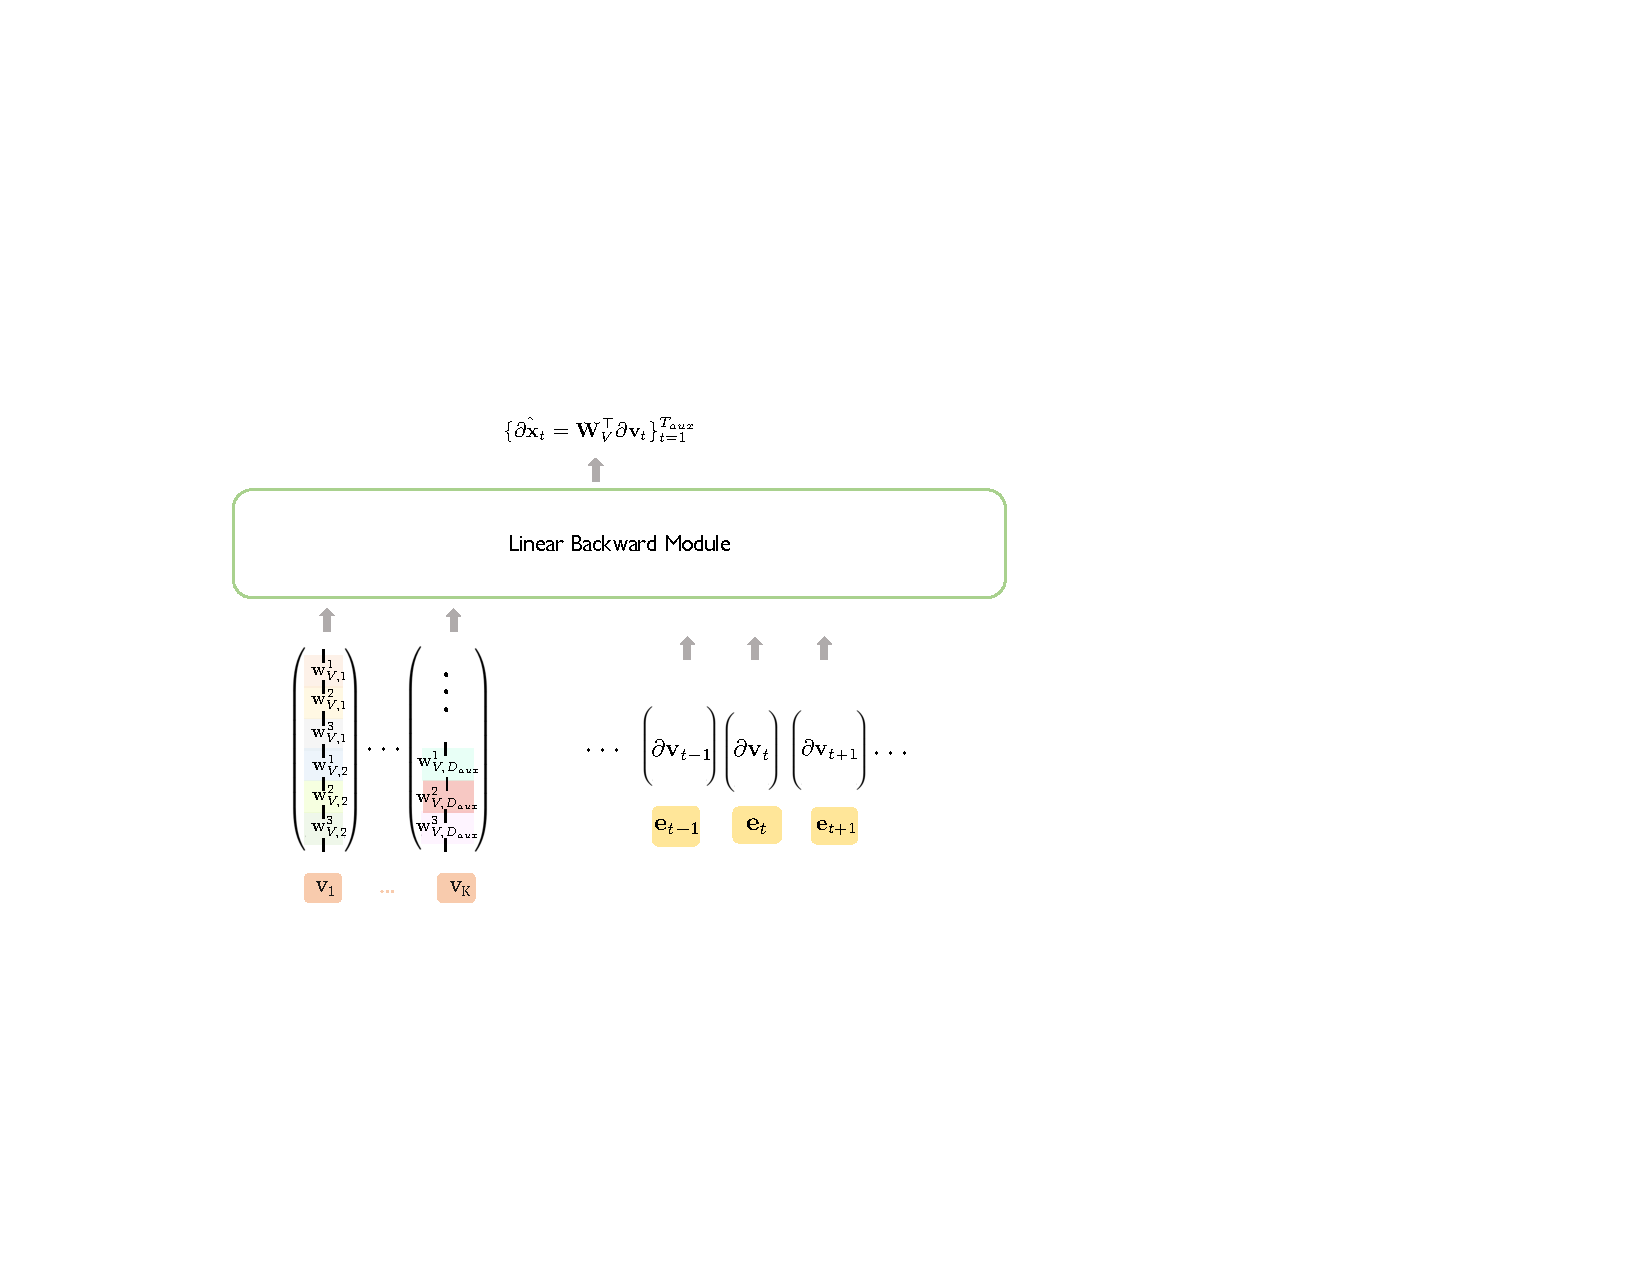
\includegraphics[width=0.75\textwidth]{figures/Attn_back.pdf}
    \caption{\simulator{} simulates the backward pass of a self-attention layer of the auxiliary model using a Linear Backward module (\cref{fig:linear_back}). The input embeddings contain the gradient of the loss w.r.t. the value vectors ($\losspartial{\vv_t}$) computed in \cref{fig:value_gradient}. The value matrix $\mW_V$ is encoded in the prefix embeddings. We call the Linear Backward module on this sequence.}
    \label{fig:attn_back}
\end{figure}


\begin{figure}[t] 
 \centering
    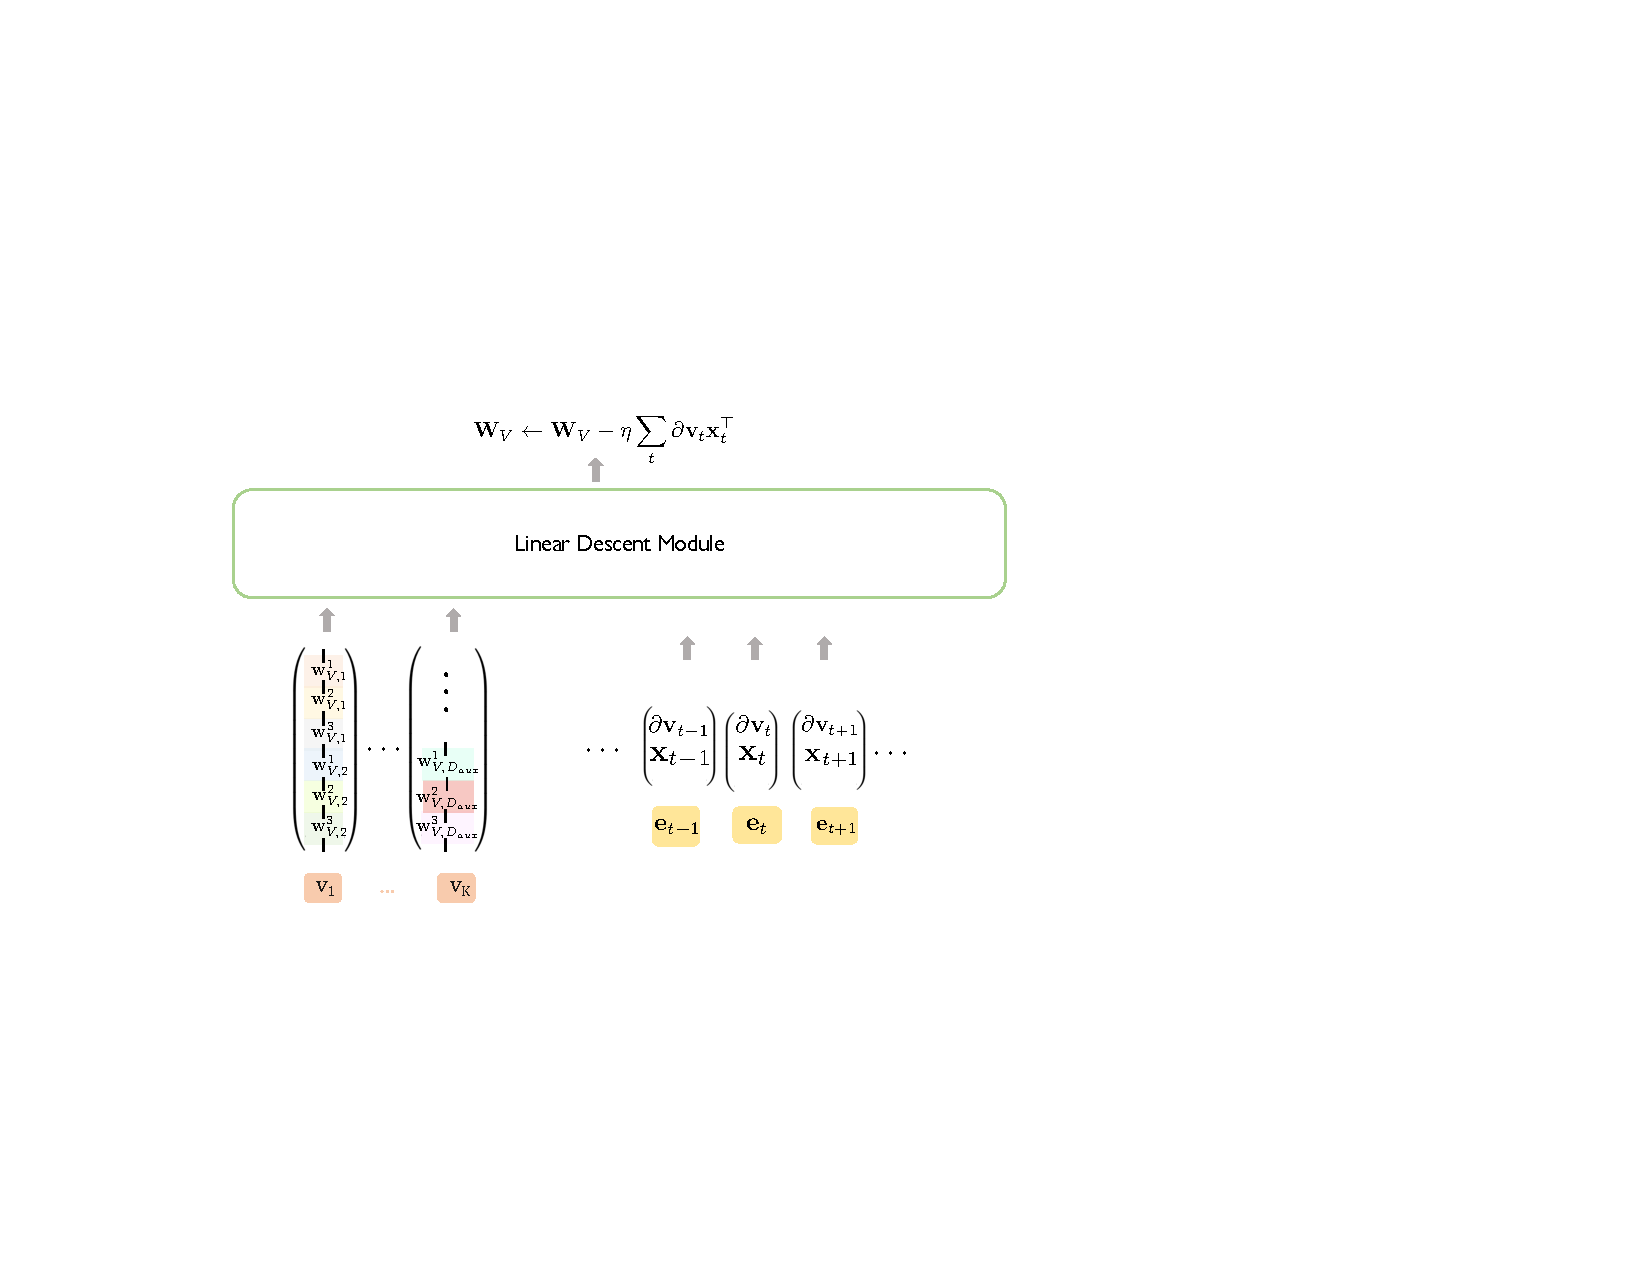
\includegraphics[width=0.75\textwidth]{figures/Attn_descent.pdf}
    \caption{ \simulator{} simulates the backward pass of the self-attention layer in the auxiliary model by employing the Linear Descent module (\cref{fig:linear_descent}). The input embeddings consist of the gradient of the loss with respect to the value vectors ($\losspartial{\vv_t}$) computed in \cref{fig:value_gradient}. Additionally, we incorporate a residual connection to copy the input from the Self-attention Forward module (\cref{fig:attn_forward}) into $\vx_t$. Before invoking the Linear Descent module, we represent the value parameters ($\mW_V$) into the prefix embeddings. \simulator{} simulates the backward pass of a self-attention layer of the auxiliary model using a Linear Descent module (\cref{fig:linear_descent}). }
    \label{fig:attn_descent}
\end{figure}



In the upcoming theorem, we formally show that if on a given sequence $\{\vx_t\}_{t \le \aux{T}}$, for all token positions all the attention heads in a self-attention layer primarily attend to a single token, then the approximate gradient $\Hat{\losspartial{\vx_t}}$ is  close to the true gradient $\losspartial{\vx_t}$ at each position $t$. 

\begin{definition}[$\varepsilon$-hard attention head]\label{def:hard_attn}
For the Self-Attention layer of $\aux{H}$ heads in \cref{def:self-attn}, on a given input sequence $\{\vx_t\}_{t=1}^{\aux{T}}$, an attention head $h \le \aux{H}$ is defined to be $\varepsilon$-hard on the input sequence, if for all positions $t \le \aux{T}$, there exists a position $t_0 \le \aux{T}$ such that $a_{t, t_0}^h \ge 1 - \varepsilon$.
\end{definition}


%\begin{definition}
%g
%\end{definition}


%\begin{theorem}\label{thm:attn_backprop}
\begin{restatable}{theorem}{boundsofthardattnt}\label{thm:attn_backprop}
With the notations in \cref{def:self-attn,def:self-attn-backprop,def:self-attn-appr-backprop}, if on a given input sequence $\{\vx_t\}_{t=1}^{\aux{T}}$, with its query, key, and value vectors $\{\vq_t, \vk_t, \vv_t\}_{t=1}^{\aux{T}}$, all the $\aux{H}$ attention heads are $\varepsilon$-hard for some $\varepsilon > 0$, then for a given sequence of gradients $\{\losspartial{\vy_t}\}_{t=1}^{\aux{T}}$, 
\begin{align*}
    \norm{\losspartial{\vq_t}}_2, \norm{\losspartial{\vk_t}}_2 \le \mathcal{O}( \varepsilon B_x^2 B^2_w B_y ), \quad \text{ for all } t \le \aux{T},
\end{align*}
where $B_x = \max_{t \le \aux{T}} \norm{\vx_t}_2$, $B_y = \max_{t \le \aux{T}} \norm{ \losspartial{\vy_t} }_2$, and $B_w = \max\{ \norm{\mW_K}_2, \norm{\mW_Q}_2, \norm{\mW_V}_2, \norm{\vb_V}_2, \norm{\vb_K}_2, \norm{\vb_V}_2 \} $.

This implies, for each position $t$, $\norm{ \Hat{\losspartial{\vx_t}} - \losspartial{\vx_t} }_2 \le \mathcal{O}(\varepsilon B_x^2 B_w^3 B_y).$
%$\max\{ \norm{\mW_K}_2, \norm{\mW_V}_2, \norm{\vb_K}_2, \norm{\vb_V}_2 \}$,  
\end{restatable}
%\end{theorem}


\paragraph{\simulator{} Self-attention backpropagation module} 
The input embeddings $\ve_t$ contain $\losspartial{\vy_t}$ in the first $\aux{D}$ coordinates.  Since we require to re-compute the attention scores $\{a^h_{t, j}\}_{j \le \aux{T}, h \le \aux{H} }$, we need to copy the query, key, and value vectors $\vq_t$, $\vk_t$, and $\vv_t$ from the \simulator{} self-attention Forward module at each position $t$. Furthermore, we use the residual connection to copy the prefix embeddings $\{ \vv_j \}$, which contain the rows of $\mW_V$, from the \simulator{} self-attention Forward module. 


The operation can be divided into three sub-operations: Computing (a) attention scores $\{ a_{t, j}^h  \}_{h \le \aux{H} }$ for all $j \le \aux{T}$, at each position $t$, (b) $\losspartial{\vv_t}$ from $\{ a_{t, j}^h  \}_{h \le \aux{H}}$ and $\losspartial{\vy_t}$, and (c) $\Hat{\losspartial{\vx_t}}$ from $\losspartial{\vv_t}$.


\begin{itemize}
    \item Sub-operation (a): Since, the current embeddings $\ve_t$ contain $\vq_t, \vk_t$, we can simply call a self-attention attention module to compute the attention scores   $\{ a_{t, j}^h  \}_{h \le \aux{H}}$ for all $j\le T$ and store them in the current embeddings. We further retain $\losspartial{\vy_t}$ and $\vv_t$ for further operations using residual connections.

    \item Sub-operation (b): With the current embeddings $\ve_t$ containing the attention scores   $\{ a_{t, j}^h  \}_{h \le \aux{H}}$ for all $j\le T$, and the gradient $\losspartial{\vy_t}$, we can compute $\losspartial{\vv_t}$ using a \simulator{} linear
 self-attention module with atleast $\aux{H}$ attention heads, that  represent the attention scores between tokens $\ve_t$ and $\ve_j$ for any $j$ as $\{ a_{j, t}^h \}_{h \le \aux{H} }$ and use $\attsplit_{ \aux{H} } ( \losspartial{\vy_t} )$ as their value vectors. 

    \item Sub-operation (c): And finally, the computation of $\Hat{\losspartial{\vx_t}}$ is identical to the  backpropagation through a linear layer, with parameters $\mW_V$ and $\vb_V$. Hence, we call a Linear backpropagation module on the current embeddings, that contain $\losspartial {\vy_t}$ and the prefix embeddings that contain $\mW_V$ and $\vb_V$.
\end{itemize}

\paragraph{Separating sub-operations (a) and (b)} The operation for computing $\losspartial{\vv_t}$ in \cref{def:self-attn-appr-backprop} looks very similar to the computation of $\vy_t$ in \cref{eq:attnt_forward}. However, the major difference is that instead of the attention scores being $\{ a_{t, j}^h \}_{h \le \aux{H} }$ between token $t$ and any token $j$, we need the attention scores to be $\{ a_{j, t}^h \}_{h \le \aux{H} }$. Thus, unless our model allows a transpose operation on the attention scores, we need to first store them in our embeddings and then use an additional self-attention module that can pick the right attention scores between tokens using position embeddings. Please see \cref{fig:attn_back}.




%\paragraph{Value parameter update}
\paragraph{Auxiliary's value descent update} Similar to the complexity of true backpropagation, the descent updates for $\mW_Q, \vb_Q, \mW_K, \vb_K$ are quite expensive to express with the transformer layers. Hence, we focus simply on updating on $\mW_V, \vb_V$, while keeping the others fixed. 


\begin{definition}[Auxiliary self-attention value descent]\label{def:self-attn-value-update}
For query, key, and value weights $\mW_Q, \mW_K, \mW_V \in\RR^{\aux{D}\times \aux{D}}$ and bias $\vb_{Q}, \vb_{K}, \vb_{V} \in\RR^{\aux{D}}$, the value descent layer corresponding to a self-attention layer with $\aux{H}$ attention heads and any function $f_{\mathrm{attn}}: \RR^{\aux{T}} \to \RR^{\aux{T}}$ takes in a batch of gradients $\{ \losspartial{ \vy_t } \in\RR^{\aux{D}} \}_{t \le \aux{T}}$ and inputs $ \{  \vx_t  \in\RR^{\aux{D}} \}_{t \le \aux{T} } $ and updates $\mW_V, \vb_V$ as follows:
\begin{align*}
&\mW_V \gets \mW_V - \eta \sum_{t \le \aux{T} } \losspartial{ \vv_t } \vx_t^{\top}, \quad \vb_V \gets \vb_V - \eta \sum_{t \le \aux{T} } \losspartial{ \vv_t }, \\& \text{ where } \losspartial{ \vv_t } = \attmerge(\{ \sum_{j} a^h_{j, t}  \losspartial{\vy^h_j} \}_{h \le \aux{H} } ) 
\end{align*} 
Here, $\vv_t$ refers to value vectors at each position $t$, as defined in \cref{def:self-attn}. 
\end{definition}


\paragraph{\simulator{} Self-attention descent module} 
The input embeddings contain $\losspartial{\vv_t}$ in the first $\aux{D}$ coordinates, from the \simulator{} self-attention backpropagation module. Furthermore, the prefix embeddings $\{ \vv_j \}$ contain the stacked rows of $\mW_V$ and $\vb_V$, continuing from the \simulator{} self-attention backpropagation module.

Since we further need the input $\vx_t$ to the auxiliary self-attention layer under consideration, we use residual connections to copy $\vx_t$ from the \simulator{} self-attention Forward module at each position $t$. 


The updates of $\mW_V$ and $\vb_V$ are equivalent to the parameter update in a linear layer, involving gradients $\{ \losspartial{\vv_t} \}$ and input $\{ \vx_t \}$. Thus, we call a Linear descent module on the current embeddings and the prefix embeddings to get the updated value parameters. Please see \cref{fig:attn_descent}.



\subsection{Proofs of theorems and gradient definitions}
We restate the theorems and definitions, before presenting their proofs for easy referencing.

\defselfattnbackprop*
\begin{proof}[Derivation of gradient in \cref{def:self-attn-backprop}]
    Recalling the definition of $\vy_t$ from \cref{def:self-attn},
    \begin{align*}
        &\vy_t = \attmerge ( \{ \sum_{j \le \aux{T}} a^h_{t, j}  \vv^{h}_j  \}_{h \le \aux{H}} ); \quad
        a^h_{t, j} =  \mathrm{softmax} ( \mK^{h} \vq^{h}_t )_j, \\&
        \vq_t = \mW_Q \vx_t + \vb_Q  \quad \vk_t =  \mW_K \vx_t + \vb_K, \quad \vv_t = \mW_V \vx_t + \vb_V.
    \end{align*}
    $\vq^{h}_t, \vk^{h}_t, \vv^{h}_t$ denote $\attsplit_{\aux{H}} (\vq_t)_h$, $\attsplit_{\aux{H}} (\vk_t)_h$, and $\attsplit_{\aux{H}} (\vv_t)_h$ respectively for all $t \le \aux{T}$, and $h \le \aux{H}$. 
     $\mK^h \in \RR^{\aux{T} \times \aux{D} }$ is defined with its rows as $\{\vk^h_t\}_{t \le \aux{T}}$ for all $h \le \aux{H}$.
    

    We explain the proof for an arbitrary token position $t$.
    With the application of the chain rule, we have
    \begin{align*}
        \losspartial{\vx_t} &= ( \frac{ \partial \vq_t }{ \partial \vx_t } )^{\top}  \losspartial{\vq_t} +   ( \frac{ \partial \vk_t }{ \partial \vx_t } )^{\top}  \losspartial{\vk_t} +
        ( \frac{ \partial \vv_t }{ \partial \vx_t } )^{\top}  \losspartial{\vv_t} \\&
        = \mW_Q^{\top} \losspartial{\vq_t} + \mW_K^{\top} \losspartial{\vk_t} + \mW_V^{\top} \losspartial{\vv_t},
    \end{align*}
    where the second step follows from the definitions of $\vq_t, \vk_t, $ and $\vv_t$ respectively.

    \paragraph{Computation of $ \losspartial {\vq_t}$: } 
    With the $\attsplit$ operation of $\vq_t$ across $\aux{H}$ heads for the computation of $\vy_t$, the computation of the backpropagated gradient $\losspartial{\vq_t}$ itself needs to be split across $\aux{H}$ heads. Furthermore, query vector $\vq_t$ only affects $\vy_t$, implying $\frac{ \partial \vy_{t'}}{\partial \vq_t} = 0$ for any $t' \ne t$.
    Thus, we have for any head $h \le \aux{H}$, if $\vy_t^h$ represents the output of attention head $h$, given by $\sum_{j \le \aux{T}} a^h_{t, j} \vv_j^h$, 
    \begingroup
    \allowdisplaybreaks
    \begin{align}
        \losspartial{\vq_t^h} &= ( \frac{ \partial \vy_t^h }{ \partial \vq_t^h } )^{\top} \losspartial{\vy_t^h} \nonumber \\
        &= \sum_{j \le \aux{T}}  \langle \vv_j^h, \losspartial{\vy_t^h} \rangle \frac{ \partial a^h_{t, j} }{ \partial \vq_t^h } \nonumber  \\ &= 
        \sum_{j \le \aux{T}}  \langle \vv_j^h, \losspartial{\vy_t^h} \rangle \frac{ \partial }{ \partial \vq_t^h } \left( \frac{ e^{ \langle \vk_j^h , \vq_t^h \rangle }  }{ \sum_{t' \le \aux{T}} e^{  \langle \vk_{t'}^h , \vq_t^h \rangle } } \right) \label{eq:softmax_expand}  \\
        &= \sum_{j \le \aux{T}}  \langle \vv_j^h, \losspartial{\vy_t^h} \rangle  \left[   \frac{1}{ \sum_{t' \le \aux{T}} e^{  \langle \vk_{t'}^h , \vq_t^h \rangle }  } \frac{ \partial e^{ \langle \vk_j^h , \vq_t^h \rangle } }{ \partial \vq_t^h }  -  \left( \frac{ e^{ \langle \vk_j^h , \vq_t^h \rangle }  }{ (\sum_{t' \le \aux{T}} e^{  \langle \vk_{t'}^h , \vq_t^h \rangle })^2  }\right)  \sum_{j' \le \aux{T}} \frac{ \partial e^{ \langle \vk_{j'}^h , \vq_t^h \rangle } }{ \partial \vq_t^h }  \right]
        \label{eq:query_expand_fractionderivation} \\
        &= \sum_{j \le \aux{T}}  \langle \vv_j^h, \losspartial{\vy_t^h} \rangle  \left[  \left( \frac{ e^{ \langle \vk_j^h , \vq_t^h \rangle }  }{ \sum_{t' \le \aux{T}} e^{  \langle \vk_{t'}^h , \vq_t^h \rangle } } \right) \vk_j^h  - \left( \frac{ e^{ \langle \vk_j^h , \vq_t^h \rangle }  }{ \sum_{t' \le \aux{T}} e^{  \langle \vk_{t'}^h , \vq_t^h \rangle } } \right) \sum_{j' \le \aux{T}} \left( \frac{ e^{ \langle \vk_{j'}^h , \vq_t^h \rangle }  }{ \sum_{t' \le \aux{T}} e^{  \langle \vk_{t'}^h , \vq_t^h \rangle } } \right) \vk^h_{j'}  \right] \label{eq:query_expanded_fractionderivation}  \\&
        = \sum_{j \le \aux{T}}  a^h_{t, j} \langle \vv_j^h, \losspartial{\vy_t^h} \rangle \left( \vk_j^h - \sum_{j' \le \aux{T}} a^h_{t, j'}  \vk^h_{j'} \right). \nonumber 
    \end{align}
    \endgroup
    
    In \cref{eq:softmax_expand}, we have expanded the definition of $\mathrm{softmax}$ in $a^h_{t, j} := \mathrm{softmax}(\mK^h \vq_t^h)_j$ in order to better motivate the derivative of $a^h_{t, j}$ w.r.t. $\vq_t^h$. Finally, $\losspartial{\vq_t}$ is given by $\attmerge(\{ \losspartial{ \vq_t^h } \}_{ h \le \aux{H} } ).$
    
    \paragraph{Computation of $ \losspartial {\vk_t}$: } Continuing as the computation of $\losspartial {\vq_t}$, we split the computation of $ \losspartial {\vk_t} $ across the $\aux{H}$ attention heads. However, unlike $\vq_t$, $\vk_t$ affects $\vy_{j}$ for all $j \le \aux{T}$. For any head $h \le \aux{H}$, we follow the chain-rule step by step to get
    \begingroup
    \allowdisplaybreaks
    \begin{align}
        \losspartial{\vk_t^h} &= \sum_{ j \le \aux{T} } ( \frac{ \partial \vy_{j}^h }{ \partial \vk_t^h } )^{\top} \losspartial{\vy_j^h} = \sum_{ j \le \aux{T} } \left( \frac{ \partial \sum_{j' \le \aux{T}} a_{j, j'} \vv_{j'}^h  }{ \partial \vk_t^h } \right)^{\top} \losspartial{\vy_j^h} \nonumber \\
        &= \sum_{ j \le \aux{T} } \langle \vv_t^h, \losspartial{\vy_{j}^h} \rangle \frac{ \partial a^h_{j, t} }{ \partial \vk_t^h }  + \sum_{j \le \aux{T}} \sum_{ j' \le \aux{T}; j' \ne t } \langle \vv_{j'}^h, \losspartial{\vy_{j}^h} \rangle \frac{ \partial a^h_{j, j'} }{ \partial \vk_t^h } \label{eq:sep_t_nott} \\
        &=   \sum_{ j \le \aux{T} } \langle \vv_t^h, \losspartial{\vy_{j}^h} \rangle \frac{ \partial }{ \partial \vk_t^h } \left( \frac{ e^{ \langle \vk_t^h, \vq_j^h \rangle } }{ \sum_{t' \le \aux{T}} e^{ \langle \vk_{t'}^h, \vq_j^h \rangle } }  \right) \label{eq:sumt_step1}\\&
        + \sum_{ j \le \aux{T} } \sum_{ j' \le \aux{T}; j' \ne t } 
 \langle \vv_{j'}^h, \losspartial{\vy_{j}^h} \rangle \frac{ \partial }{ \partial \vk_t^h } \left( \frac{ e^{ \langle \vk_{j'}^h, \vq_j^h \rangle } }{ \sum_{t' \le \aux{T}} e^{ \langle \vk_{t'}^h, \vq_j^h \rangle } }  \right)  \label{eq:sumnott_step1}\\&
= \sum_{ j \le \aux{T} } \langle \vv_t^h, \losspartial{\vy_{j}^h} \rangle \left[ \left( \frac{ e^{ \langle \vk_t^h, \vq_j^h \rangle } }{ \sum_{t' \le \aux{T}} e^{ \langle \vk_{t'}^h, \vq_j^h \rangle } }  \right) \vq_j^h - \left( \frac{ e^{ \langle \vk_t^h, \vq_j^h \rangle } }{ \sum_{t' \le \aux{T}} e^{ \langle \vk_{t'}^h, \vq_j^h \rangle } }  \right)^2  \vq_{j}^h \right]  \label{eq:sumt_step2}\\&
 - \sum_{ j \le \aux{T} } \sum_{ j' \le \aux{T}; j' \ne t } \langle \vv_{j'}^h, \losspartial{\vy_{j}^h}  \rangle \left( \frac{ e^{ \langle \vk_{j'}^h, \vq_j^h \rangle } }{ \sum_{t' \le \aux{T}} e^{ \langle \vk_{t'}^h, \vq_j^h \rangle } }  \right) \left( \frac{ e^{ \langle \vk_t^h, \vq_j^h \rangle } }{ \sum_{t' \le \aux{T}} e^{ \langle \vk_{t'}^h, \vq_j^h \rangle } }  \right) \vq_j^h  \label{eq:sumnott_step2}\\&
 = \sum_{ j \le \aux{T} } \langle \vv_t^h, \losspartial{\vy_{j}^h} \rangle ( a^h_{j, t} - (a^h_{j, t})^2  ) \vq_j^h - \sum_{ j \le \aux{T} } \sum_{ j' \le \aux{T}; j' \ne t } \langle \vv_{j'}^h, \losspartial{\vy_{j}^h}  \rangle a^h_{j, j'} a^h_{j, t} \vq_j^h  \nonumber\\&
 = \sum_{ j \le \aux{T} }  a^h_{j, t}   \langle \losspartial{\vy_j^h},  \vv^{h}_t - \sum_{j'} a^h_{j, j'} \vv^{h}_{j'} \rangle   \vq^{h}_{j}  \nonumber
    \end{align}
    \endgroup

In \cref{eq:sep_t_nott}, we separate the inside sum into two components, since the derivative w.r.t. $\vk_t^h$ differ for the two components, as outlined in the derivation of \cref{eq:sumt_step2} from \cref{eq:sumt_step1}, and \cref{eq:sumnott_step2} from \cref{eq:sumnott_step1}. We have skipped a step going from  \cref{eq:sumnott_step1,eq:sumt_step1} to  \cref{eq:sumt_step2,eq:sumnott_step2} due to typographical simplicity. The skipped step is extremely similar to \cref{eq:query_expand_fractionderivation} in the derivation of $\losspartial{\vq_t^h}.$ Finally, $\losspartial{\vk_t}$ is given by $\attmerge(\{ \losspartial{ \vk_t^h } \}_{ h \le \aux{H} } ).$
    


\paragraph{Computation of $ \losspartial {\vv_t}$:} Similar to the gradient computation of $\vq_t$, the computation of $ \losspartial {\vv_t} $ needs to be split across the $\aux{H}$ attention heads. However, like $\vk_t$, $\vv_t$ affects $\vy_j$ for all $j \le \aux{T}$. For any head $h \le \aux{H}$, we follow the chain-rule step by step to get
\begin{align*}
    \losspartial{\vv_t^h} &= \sum_{ j \le \aux{T} } ( \frac{ \partial \vy_{j}^h }{ \partial \vv_t^h } )^{\top} \losspartial{\vy_j^h}  = \sum_{ j \le \aux{T} } \left( \frac{ \partial \sum_{j' \le \aux{T}} a_{j, j'} \vv_{j'}^h  }{ \partial \vv_t^h } \right)^{\top} \losspartial{\vy_j^h} 
    = \sum_{ j \le \aux{T} } a_{j, t}^h \losspartial{\vy_j^h}
\end{align*}


\end{proof}




\boundsofthardattnt*
\begin{proof}[Proof of \cref{thm:attn_backprop}]
    For typographical simplicity, we discuss the proof at an arbitrary position $t$. Recall the definition of an $\varepsilon$-hard attention head from \cref{def:hard_attn}. An attention head is defined to be $\varepsilon$-hard on an input sequence $\{ \vx_t \}_{t=1}^{\aux{T}}$, if for each position $t$, there exists a position $t_0$ such that the attention score $a_{t, t_0} \ge 1 - \varepsilon$.
    
    
    For the proof, we simply focus on $\losspartial{\vq_t}$, and the proof for $\losspartial{\vk_t}$ follows like-wise. 
    \paragraph{Bounds on $\vq_t$:}
    Recalling the definition of $\losspartial{\vq_t}$ from \cref{def:self-attn-backprop}, we have
    \begin{align*}
        \losspartial{ \vq_t } =  \attmerge( \{  \sum_j a^h_{t, j} ( (\losspartial{\vy_t^h})^{\top} \vv^{h}_j ) [ \vk^h_j - \sum_{j'} a^h_{t, j'} \vk^{h}_{j'} ]  \}_{h \le \aux{H}} ).
    \end{align*}
    
    Focusing on a head $h \le \aux{H}$, define $\losspartial{ \vq_t^h } = \sum_j a^h_{t, j} ( (\losspartial{\vy_t^h})^{\top} \vv^{h}_j ) [ \vk^h_j - \sum_{j'} a^h_{t, j'} \vk^{h}_{j'} ]$ and $t_0 \le \aux{T}$ as the token position where the $\vq_t$ attends the most to, i.e. $a^h_{t, t_0} \ge 1 - \varepsilon$ and $\sum_{j \le \aux{T}; j \ne t_0} a^h_{t, j} \le \varepsilon$. Then,
    \begin{align*}
        \norm{ \losspartial { \vq^h_t } }_2 &= \norm{ \sum_j a^h_{t, j} ( (\losspartial{\vy_t^h})^{\top} \vv^{h}_j ) [ \vk^h_j - \sum_{j'} a^h_{t, j'} \vk^{h}_{j'} ] }_2 \\&
        = \norm{ a^h_{t, t_0} ( (\losspartial{\vy_t^h})^{\top} \vv^{h}_{t_0} ) [ \vk^h_{t_0} - \sum_{j'} a^h_{t, j'} \vk^{h}_{j'} ]  + \sum_{j \ne t_0} a^h_{t, j} ( (\losspartial{\vy_t^h})^{\top} \vv^{h}_j ) [ \vk^h_j - \sum_{j'} a^h_{t, j'} \vk^{h}_{j'} ] }_2  \\&
        \leq \underbrace{\norm{ a^h_{t, t_0} ( (\losspartial{\vy_t^h})^{\top} \vv^{h}_{t_0} ) [ \vk^h_{t_0} - \sum_{j'} a^h_{t, j'} \vk^{h}_{j'} ] }_2}_{\mathrm{Term 1}} + \underbrace{\norm{ \sum_{j \ne t_0} a^h_{t, j} ( (\losspartial{\vy_t^h})^{\top} \vv^{h}_j ) [ \vk^h_j - \sum_{j'} a^h_{t, j'} \vk^{h}_{j'} ] }_2}_{\mathrm{Term 2}}, 
    \end{align*}
    where the final step uses a Cauchy-Schwartz inequality. We focus on the two terms separately.

    \begin{enumerate}
        \item $\mathrm{Term 1}$: Focusing on $\vk^h_{t_0} - \sum_{j'} a^h_{t, j'} \vk^{h}_{j'}$, we have
        \begin{align}
            \norm{\vk^h_{t_0} - \sum_{j'} a^h_{t, j'} \vk^{h}_{j'}}_2 &= \norm{ (1 - a_{t, t_0}) \vk^h_{t_0} - \sum_{j' \ne t_0} a^h_{t, j'} \vk^{h}_{j'} }_2 \nonumber\\&
            \leq (1 - a_{t, t_0}) \norm{ \vk^h_{t_0} }_2 + \sum_{j' \ne t_0}  a^h_{t, j'} \norm{ \vk^{h}_{j'} }_2 \nonumber\\&
            \leq  ( (1 - a_{t, t_0}) + \sum_{j' \ne t_0}  a^h_{t, j'} ) \max_{j} \norm{ \vk^h_j }_2 \nonumber\\&
            \leq 2 \varepsilon \max_{j} \norm{ \vk^h_j }_2 \label{eq:bound_on_diffk}.
        \end{align}
        We use a Cauchy-Schwartz inequality in the second and third steps and the attention head behavior in the final step.

        Hence, $\mathrm{Term 1}$ can now be bounded as follows:
        \begin{align*}
            \norm{ a^h_{t, t_0} ( (\losspartial{\vy_t^h})^{\top} \vv^{h}_{t_0} ) [ \vk^h_{t_0} - \sum_{j'} a^h_{t, j'} \vk^{h}_{j'} ] }_2 &=  a^h_{t, t_0}  \abs{ (\losspartial{\vy_t^h})^{\top} \vv^{h}_{t_0} } \norm{  \vk^h_{t_0} - \sum_{j'} a^h_{t, j'} \vk^{h}_{j'} }_2, \\&
            \leq 2 \varepsilon \norm{ \losspartial{\vy_t^h} }_2 \norm{ \vv^{h}_{t_0} }_2   \max_{j} \norm{ \vk^h_j }_2.
        \end{align*}
        In the final step, in addition to the bound from \cref{eq:bound_on_diffk}, we use a  Cauchy-Schwartz inequality to bound $\abs{ (\losspartial{\vy_t^h})^{\top} \vv^{h}_{t_0} }$ and bound the attention score $a^h_{t, t_0} $ by $1$.
        
        \item $\mathrm{Term 2}$: Focusing on $\vk^h_{j} - \sum_{j'} a^h_{t, j'} \vk^{h}_{j'}$ for any $j \le \aux{T}$, we have using two Cauchy-Schwartz inequalities:
        \begin{align}
            \norm{\vk^h_{j} - \sum_{j'} a^h_{t, j'} \vk^{h}_{j'}}_2 &\leq \norm{\vk^h_j}_2 + \norm{ \sum_{j'} a^h_{t, j'} \vk^{h}_{j'} }_2 
            \leq (1 + \sum_{j'} a^h_{t, j'}) \max_{j'} \norm{ \vk^{h}_{j'} }_2  = 2 \max_{j'} \norm{ \vk^{h}_{j'} }_2 \label{eq:bound_k_j_diff}. 
        \end{align}
        Hence,
        \begin{align*}
            \norm{ \sum_{j \ne t_0} a^h_{t, j} ( (\losspartial{\vy_t^h})^{\top} \vv^{h}_j ) [ \vk^h_j - \sum_{j'} a^h_{t, j'} \vk^{h}_{j'} ] }_2 &\leq  \left( \sum_{ j \ne t_0 } a^h_{t, j} \right) \max_j \abs{ (\losspartial{\vy_t^h})^{\top} \vv^{h}_j }  \norm{ \vk^h_j - \sum_{j'} a^h_{t, j'} \vk^{h}_{j'} }_2 \\&
            \leq 2\varepsilon \norm{ \losspartial{ \vy_t^h } }_2 \left( \max_j \norm{ \vv_j^h }_2 \right) \left( \max_{j'} \norm{ \vk^{h}_{j'} }_2 \right)
            .
        \end{align*}
        In the final step, in addition to the bound from \cref{eq:bound_k_j_diff}, we use a  Cauchy-Schwartz inequality to bound $\abs{ (\losspartial{\vy_t^h})^{\top} \vv^{h}_j }$ and use the $\varepsilon$-hard behavior of the attention head to bound $\sum_{j \ne t_0} a^h_{t, j}.$
        
        
    \end{enumerate}
    Combining the bounds on both terms, we have
    \begin{align*}
        \norm{ \losspartial { \vq^h_t } }_2 &\leq 2 \varepsilon \norm{ \losspartial{\vy_t^h} }_2 \norm{ \vv^{h}_{t_0} }_2   \max_{j} \norm{ \vk^h_j }_2 + 2\varepsilon \norm{ \losspartial{ \vy_t^h } }_2 \left( \max_j \norm{ \vv_j^h }_2 \right) \left( \max_{j'} \norm{ \vk^{h}_{j'} }_2 \right) \\& \leq 4 \varepsilon \norm{ \losspartial{ \vy_t^h } }_2 \left( \max_j \norm{ \vv_j^h }_2 \right) \left( \max_{j'} \norm{ \vk^{h}_{j'} }_2 \right).
    \end{align*}
    We bound the remaining terms as follows.
    \begin{itemize}
        \item $\norm{ \losspartial{ \vy_t^h } }_2 \le B_y$, under the bounded assumption of the gradients.

        \item For any $j \le \aux{T}$, we have $\norm{ \vk_j^{h} }_2 \leq \norm{ \vk_j }_2$ since $\vk_j = \attmerge( \{ \vk_j^{h'} \}_{h' \in \aux{H} } )$. Furthermore, from the defintion of the key vector $\vk_j$, $\norm{ \vk_j }_2 = \norm{ \mW_K \vx_j + \vb_K }_2 \leq \norm{\mW_K}_2 \norm{\vx_j}_2 + \norm{\vb_K}_2$ with a Cauchy-Schwartz inequality. Under the bounded assumptions of $\mW_K, \vb_K$ and input $\vx_j$, we have $\norm{ \vk_j }_2 \leq B_w(1 + B_x).$

        \item Similar procedure can be followed for bounding $ \max_j \norm{ \vv_j^h }_2$. 
    \end{itemize}

    Thus, we have $\norm{ \losspartial { \vq^h_t } }_2 \leq 4 \varepsilon \norm{ \losspartial{ \vy_t^h } }_2 \left( \max_j \norm{ \vv_j^h }_2 \right) \left( \max_{j'} \norm{ \vk^{h}_{j'} }_2 \right) \leq 4 \varepsilon B^2_w (1 + B_x)^2 B_y.$
    

    \paragraph{Bounds on $\norm{\Hat{\losspartial{\vx_t}} - \losspartial{\vx_t}}_2$:}
    From the definitons of $\Hat{\losspartial{\vx_t}}$ and $\losspartial{\vx_t}$ from \cref{def:self-attn-appr-backprop,def:self-attn-appr-backprop}, we have
    
    \begin{align*}
        \norm{\Hat{\losspartial{\vx_t}} - \losspartial{\vx_t}}_2 
        &= \norm{ \mW_K^{\top} \losspartial{\vk_t} + \mW_Q^{\top} \losspartial{\vq_t} }_2 \leq \norm{ \mW_K }_2 \norm{ \losspartial{\vk_t} }_2 +  \norm{ \mW_Q }_2 \norm{ \losspartial{\vq_t} }_2
        \\& \leq 8 \varepsilon B^3_w (1 + B_x)^2 B_y = \mathcal{O}(  \varepsilon B^3_w  B_x^2 B_y ),
    \end{align*}
    where we use Cauchy-schwartz inequality in the second step. We use the assumed bounds on $\norm{ \mW_Q }_2, \norm{ \mW_K }_2$, and the computed bounds on $\norm{ \losspartial{\vq_t} }_2, \norm{ \losspartial{\vk_t} }_2$ in the pre-final step.
\end{proof}


